\begin{solutionfigure}[htb]
    \centering
    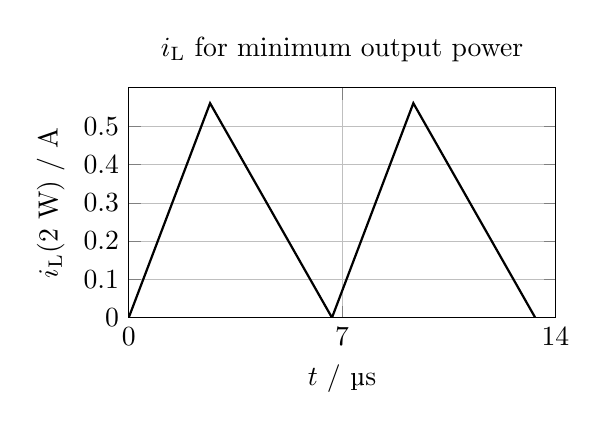
\begin{tikzpicture}
    \begin{axis}[
        width=7cm, height=4.5cm,
        grid=both,
        major grid style={line width=.2pt,draw=gray!50},
        minor grid style={line width=.1pt,draw=gray!20},
        xlabel={$t$ / µs},
        ylabel={$i_\mathrm{L}(\mathrm{2~W})$ / A},
        title={$i_\mathrm{L}$ for minimum output power},
        xmin=0, xmax=14,
        ymin=0, ymax=0.6,
        xtick={0, 7, 14},
        ytick={0, 0.1, 0.2, 0.3, 0.4, 0.5},
        ]
        % Einschaltverhalten graph
        \addplot[
            thick,
            mark=none,
            color=black,
        ] coordinates {
            (0,0) (2.67,0.56) (6.67, 0) (9.34,0.56) (13.34, 0)
        };
    \end{axis}
    \end{tikzpicture} 
    \hspace{1cm} % Abstand zwischen den beiden Diagrammen
    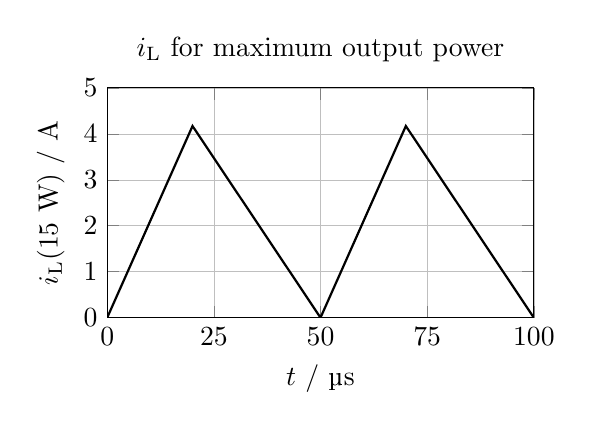
\begin{tikzpicture}
    \begin{axis}[
        width=7cm, height=4.5cm,
        grid=both,
        major grid style={line width=.2pt,draw=gray!50},
        minor grid style={line width=.1pt,draw=gray!20},
        xlabel={$t$ / µs},
        ylabel={$i_\mathrm{L}(\mathrm{15~W})$ / A},
        title={$i_\mathrm{L}$ for maximum output power},
        xmin=0, xmax=100,
        ymin=0, ymax=5,
        xtick={0, 25, 50, 75, 100},
        ytick={0, 1, 2, 3, 4, 5},
        ]
        % Ausschaltverhalten graph
        \addplot[
            thick,
            mark=none,
            color=black,
        ] coordinates {
            (0,0) (20, 4.17) (50, 0) (70, 4.17) (100, 0)
        };
    \end{axis}
    \end{tikzpicture}
    \caption{Display of the current $i_\mathrm{L}$ for minimum and maximum output power.}
    \label{fig:InductorCurrentEx03}
    \end{solutionfigure}